\documentclass[11pt]{article}
\usepackage{Fall24/classTools}
\usepackage{graphicx}
\drafttrue

\begin{document}
\psHeader{0}{Wed 2024-09-11 (11:59PM)}

The purpose of this problem set is to reactivate your skills in proofs and programming from CS20 and CS32/CS50. For those of you who haven't taken one or both those courses, the problem set can also help you assess whether you have acquired sufficient skills to enter CS1200 in other ways and can fill in any missing gaps through self-study. Even for students with all of the recommended background, this problem set may still require a significant amount of thought and effort, so do not be discouraged if that is the case and do take advantage of the staff support in section and office hours. 

For those of you who are wondering whether you should wait and take CS20 before taking CS1200, we encourage you to also complete  \href{https://drive.google.com/file/d/1QIJR6sb9hfkK67PhpQaK9KQBzYwzXvsW/view}{the CS20 Placement Self-Assessment}.  Some problems there that are of particular relevance to CS1200 are Problems 2 (counting), 4 \& 5 (comparing growth rates), 9 (quantificational logic), and 12 (graph theory). 

Written answers must be submitted in pdf format on Gradescope. Although \LaTeX{} is not required, it is strongly encouraged. You may handwrite solutions so long as they are fully legible. The \texttt{ps0} directory, which contains your code for problems 1a and 1c, must be submitted separately to an autograder on Gradescope. Please fill out the ``GitHub Username Submission" assignment on Gradescope to be added to the GitHub Classroom assignment - in the meantime, you can accept the \href{https://classroom.github.com/a/BwZDNK_r}{GitHub Classroom assignment}, or pull the starter code from the \href{https://github.com/Harvard-CS-1200/cs1200}{cs1200 GitHub repository}.

 \newcommand{\children}{\mathit{children}}
 %\renewcommand{\treeroot}{\mathit{treeroot}}
 \newcommand{\parent}{\mathit{parent}}
 
\begin{enumerate}
\item (Binary Trees) 
\iffalse 
Recall the following properties of a (rooted) {\em tree}:
    \begin{itemize}
        \item A (rooted) {\em tree} $T$ consists of a finite set $V$ of vertices (also sometimes called ``nodes''), one of which is the {\em root} $r\in V$
        \item Every vertex $v$ has a finite set $\children(v)\subseteq V-\{r\}$ of children; no two vertices $v\neq w$ share any children (i.e. $\children(v)\cap \children(w) = \emptyset$) and every vertex other than the root is the child of some vertex (i.e. $\bigcup_{v\in V} \children(v) = V-\{r\}$)
        \item For a vertex $v$ other than $r$, $\parent(v)$ is the unique vertex $w$ such that $v\in \children(w)$.
        \item A {\em leaf} of a (rooted) tree is a vertex $v$ with no children.
        \item  The {\em size} of a tree is its number of vertices.
        \item A vertex $w$ is a {\em descendant} of a vertex $v$ if there is a sequence of vertices $v_0,v_1,\ldots,v_k\in V$, $k\in \mathbb{N}$ such that $v_0=v$, $v_k=w$, and $v_i\in \children(v_{i-1})$ for $i=1,\ldots,k$.
        \footnote{$\mathbb{N}$ denotes the natural numbers $\{0,1,2,3,\ldots\}$.  Since we are computer scientists, we start counting at 0.}
        \item The sequence $(v_0,v_1,\ldots,v_k)$ is called a {\em path} from $v$ to $w$ and $k$ is the {\em distance} from $v$ to $w$.
 Taking $k=0$, we see that $v$ is a descendant of itself.
        \item Given any vertex $v$ in a tree, the {\em subtree} rooted at $v$ is the tree consisting of all of $v$'s descendants, with $v$ as the root.
        \item The {\em height} of a tree $T$ is the largest distance from the root to a leaf.
    \end{itemize}
    
 A binary tree has the additional constraint where every vertex $v$ has 0, 1, or 2 children.
\fi

 In the \href{https://github.com/Harvard-CS-1200/cs1200}{cs1200 GitHub repository}, we have given you a Python implementation of a binary tree data structure, as well as a collection of test trees built using this data structure.  We specify a binary tree by giving a pointer to its {\em root}, which is a special {\em vertex} (a.k.a. {\em node}), and giving every vertex pointers to its {\em children} vertices and its {\em parent} vertex as well as an identifying {\em key}: 
 
 \begin{verbatim}
    class BinaryTree:
        def __init__(self, root):
            self.root: BTvertex = root
 
    class BTvertex:
        def __init__(self, key):
            self.parent: BTvertex = None
            self.left: BTvertex = None
            self.right: BTvertex = None
            self.key: int = key
            self.size: int = None
 \end{verbatim}


 In CS50, the concept of a Python \texttt{class} was not covered. Here, with \texttt{BinaryTree} and \texttt{BTvertex}, we are using them in the same way as a \texttt{struct} in C. An object \btv\ of the \texttt{BTvertex} class contains five attributes, which we list with the type of the object we expect to be named by each attribute (using the Python type annotation syntax). These attributes can be accessed as \texttt{v.parent}, \texttt{v.left}, \texttt{v.right}, \texttt{v.key}, and \texttt{v.size}. 
 For example, \texttt{v.left.key} is the key associated with \btv's left child. An object of the \texttt{BinaryTree} class contains only one attribute, which is the \texttt{BTvertex} object that is the root of our binary tree. You can create a \texttt{BinaryTree} object as follows:
 
\begin{verbatim}
root = BTvertex(120)
tree = BinaryTree(root)
tree.root.left = BTvertex(121)
tree.root.right = BTvertex(124)
\end{verbatim}

You can then print attributes of the newly created \texttt{BinaryTree} object:
\begin{verbatim}
print(tree.root.key)
>> 120
print(tree.root.left.key)
>> 121
\end{verbatim}
 

 Classes are more general than structs because they can also have private attributes and methods that operate on the attributes, allowing for object-oriented programming. However, you won't need that generality in this problem set.

 Here is an instance \treeT\ of \texttt{BinaryTree}:
 
 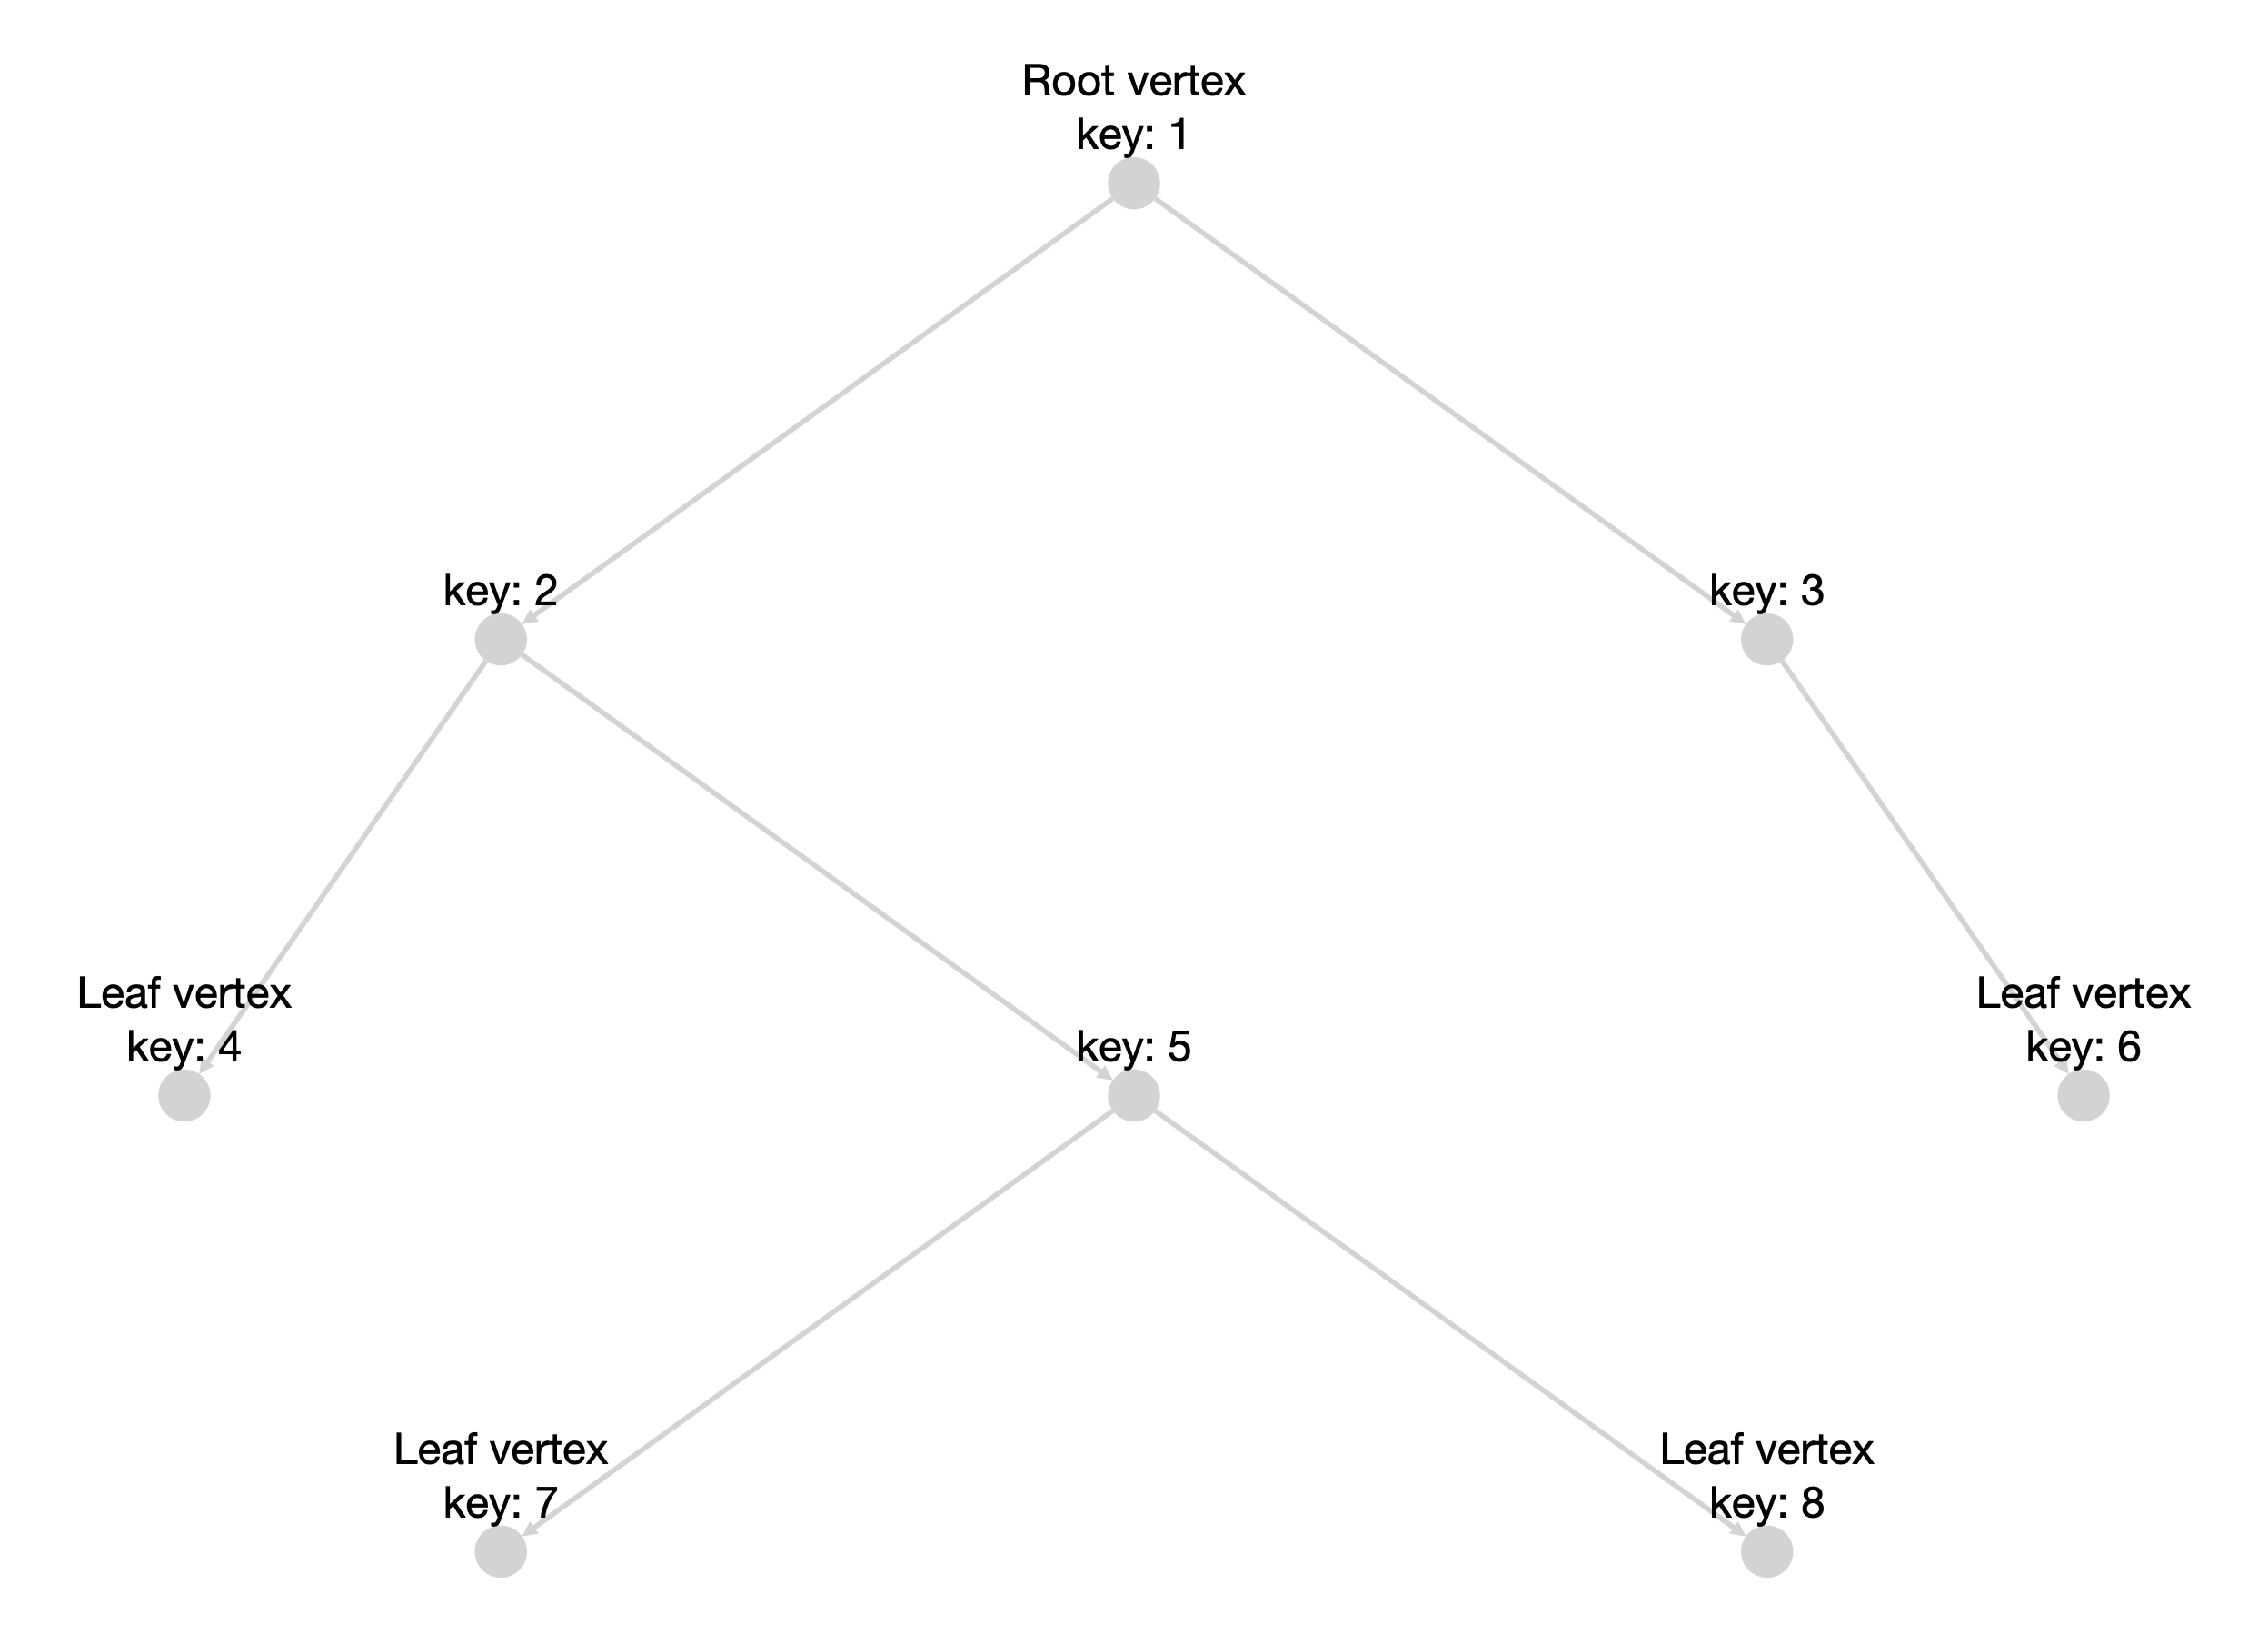
\includegraphics[scale=.175]{Fall23/Problem Sets and Exams/ps0/ps0_assets/p0_q1_BT_before.png}

 A \texttt{BinaryTree} \treeT\  contains only a pointer to its root vertex, \texttt{T.root}, which is required to satisfy \texttt{T.root.parent==None}. In the above example, 
 the root is the vertex with key 1 (i.e. \texttt{T.root.key==1}).
 A binary tree vertex \btv\ can have zero, one, or two children, determined by which of \texttt{v.left} and  \texttt{v.right} are equal to \texttt{None}.    In the above example, the vertex \btv\ with key 3 has 
 \texttt{v.left==None} but \texttt{v.right} is the vertex with key 6.
 A {\em leaf} is a vertex with zero children, i.e. \texttt{v.left==v.right==None}. 
 
 A vertex \btw\ is {\em descendant} of a vertex \texttt{v} if there is a sequence of vertices $\btv_0,\btv_1,\ldots,\btv_k$, $k\in \mathbb{N}$ such that $\btv_0=\btv$, $\btv_k=\btw$, and 
 $\btv_i \in \{\btv_{i-1}.\texttt{left},\btv_{i-1}.\texttt{right}\}$ for $i=1,\ldots,k$.\footnote{$\mathbb{N}$ denotes the natural numbers $\{0,1,2,3,\ldots\}$.  Since we are computer scientists, we start counting at 0.}
 In the above example, the vertex with key 5 is a descendant of the root (with a path of length 2), but is not a descendant of the vertex with key 3.
 The sequence $\btv_0,\btv_1,\ldots,\btv_k$ is called a {\em path} from \btv\ to \btw\ and $k$ is the {\em distance} from \btv\ to \btw. Taking $k=0$, we see that \btv\ is a descendant of itself.

 The {\em vertex set} of a binary tree \treeT\ consists of all of the descendants of \texttt{T.root}. The {\em size} of \treeT\ is its number of vertices. 
 The {\em height} of \treeT\ is the largest distance from the root to a leaf.  The above example has size 8 and height 3.
 
 Given any vertex \btv\ in a tree, the {\em subtree} rooted at \btv\ consists of all of \btv's descendants.  Note that we can remove a subtree and turn it into a new tree \texttt{S} by setting
 \texttt{S.root=v} and \texttt{v.parent=None}.

 For now, the \texttt{key} attribute serves to distinguish vertices from each other in our tests and help illustrate what the algorithms are doing.  The \texttt{BTvertex}\ class
 also has a \texttt{size} attribute, which is initialized to \texttt{None} in all of the test instances; it will be filled in by the program you write in Part~\ref{part:calculatesizes}.

 An instance \treeT\ \texttt{BinaryTree} is {\em valid} if it satisfies the following constraints: \begin{itemize}
     \item \texttt{T.root.parent==None}
     \item \treeT\ has finitely many vertices.
     \item No two vertices \btv, \btw\ of \treeT\ share a child, i.e. 
     $\{\texttt{v.left},\texttt{v.right}\} \cap \{\texttt{w.left},\texttt{w.right}\} = \emptyset$. 
 \end{itemize}
 All of the test instances we provide are valid, and furthermore have the property that all of the vertices have distinct keys (which is something we often want, but not always).

 \begin{enumerate}
 \item \label{part:calculatesizes} (recursive programming)
 Write a recursive program \texttt{calculate\_sizes} that given a vertex \btv\ of a binary tree \treeT, calculates the sizes of all of the subtrees rooted at descendants of \btv.  After running your program on \texttt{T.root}, every vertex \btv\ in \treeT\ should have \texttt{v.size} set to the size of the subtree rooted at \btv. (Recall that the size attributes are initialized to \texttt{None}.)  We call the resulting tree a {\em size-augmented} tree.
 
For example, if \treeT\  is the  tree shown above, 
then calling \texttt{calculate\_sizes(T.root)} should modify  \treeT\ to be the following size-augmented tree:

 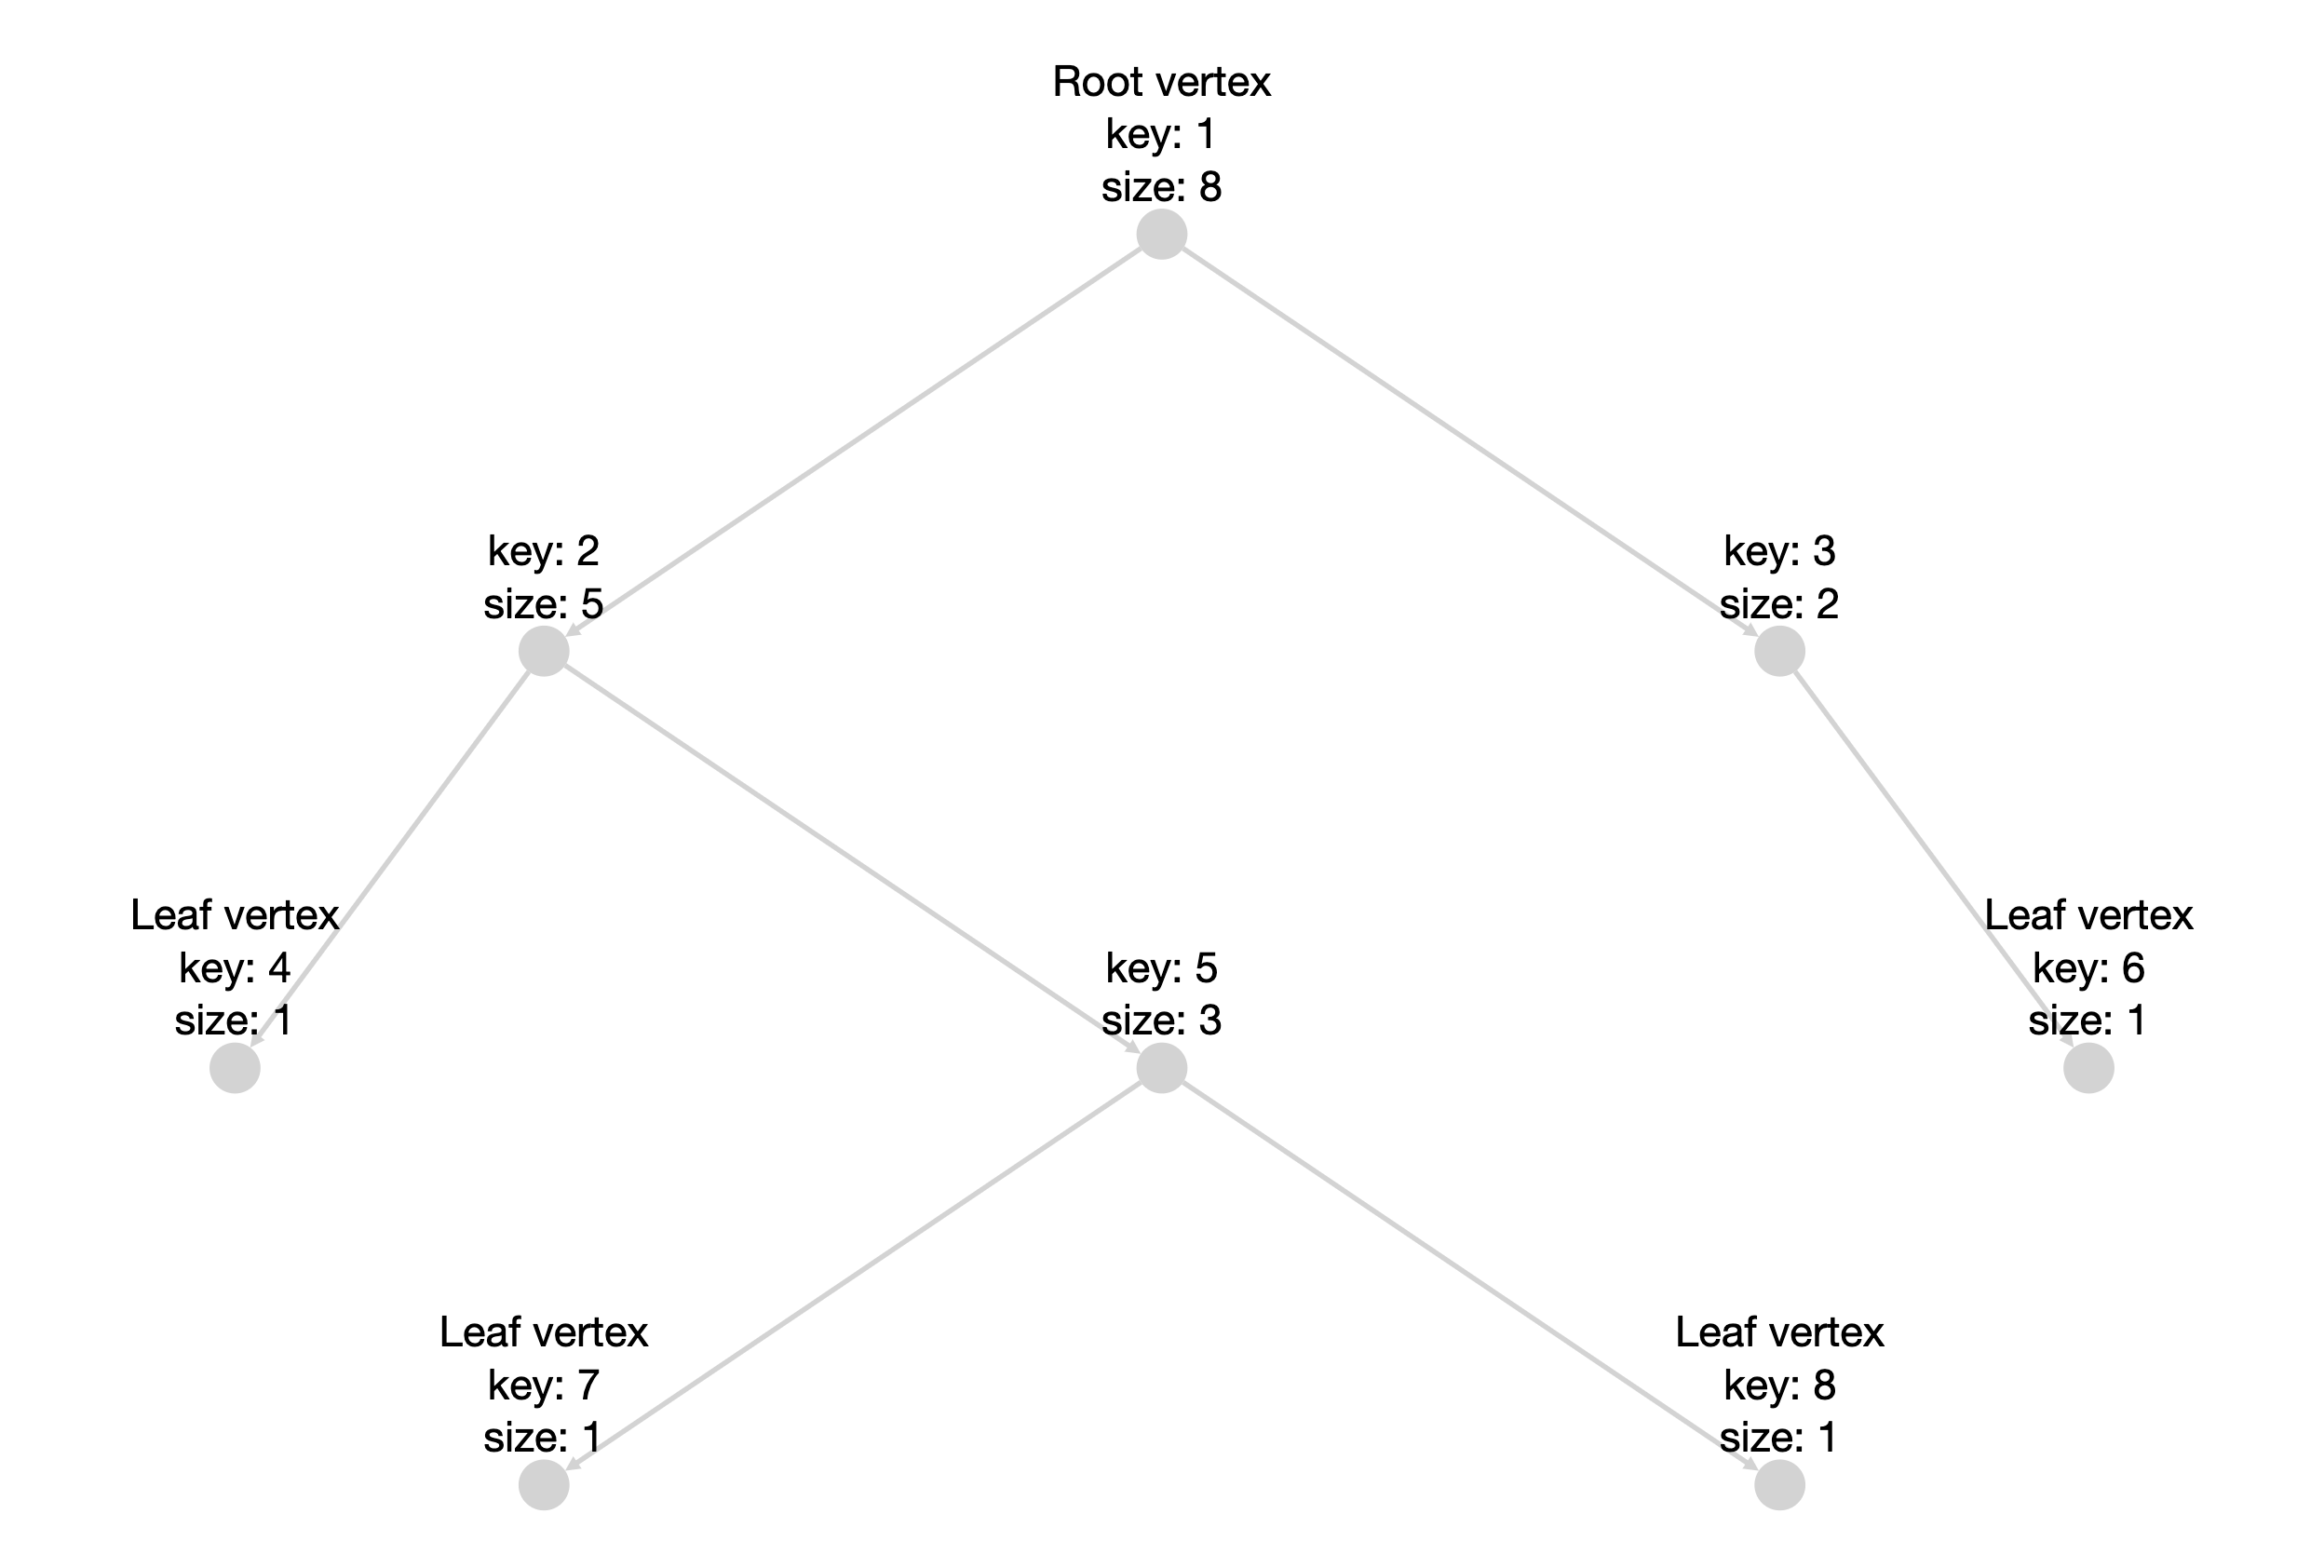
\includegraphics[scale=.175]{Fall23/Problem Sets and Exams/ps0/ps0_assets/p0_q1_BT_after.png}

 Your program should run in time $O(n)$ when given the root of a tree with $n$ vertices. In a sentence or two, informally justify why your program has such a runtime. 


    \item (proofs by induction) Let $t$ be a positive integer. Prove that every binary tree $\treeT$ of size at least $2t+1$ has a vertex $\btv$ such that the subtree rooted at $\btv$ has size at least $t$ and at most $2t$.  (Hint: use induction on the size $n$ of $\treeT$, starting with base case $n=2t+1$.  Remember that nodes in binary trees can have 2, 1, or 0 children.) \label{part:induction-tsize}
    
    \item (from proofs to algorithms) Turn your proof from Part~\ref{part:induction-tsize} into a Python program \texttt{FindDescendantOfSize(t,v)} that, given a positive integer $\texttt{t}$ and a vertex \texttt{v} of a {\em size-augmented} tree \treeT\ such that $\texttt{v.size}\geq \texttt{2t+1}$, finds and returns a descendant  \texttt{w} of $\texttt{v}$ such that $\texttt{t}\leq \texttt{w.size} \leq \texttt{2t}$.  Your algorithm should run in time $O(h)$, where $h$ is the height of the subtree rooted at $\texttt{v}$; explain in words why this is the case.
\end{enumerate}
 

\item (asymptotic notation) Recall the definitions of asymptotic notation from CS20:
Let $f$ and $g$ be functions from $\N$ to $\R^+$, where $\N=\{0,1,2,\ldots\}$ denotes the natural numbers (including 0, since we are computer scientists) and $\R^+$ denotes the positive real numbers.  
\begin{itemize}
    \item We say that $f=O(g)$ if there is a constant $c>0$ such that $f(n)\leq c\cdot g(n)$ for all sufficiently large $n$. 
    \item We say that $f=o(g)$ if for {\em every} constant $c>0$, $f(n)\leq c\cdot g(n)$ for all sufficiently large $n$; equivalently, $\lim_{n\rightarrow \infty} (f(n)/g(n))=0$.
\end{itemize}


\begin{enumerate}
    \item For each of the following pairs of functions, determine whether $f=O(g)$ and whether $f=o(g)$.  Justify your answers.
    \begin{enumerate}
        \item $f(n) = 3\log_2^3 n$, $g(n) = n^2+1$.
        \item $f(n) = 4n^3$, $g(n)= \left| \{S \subseteq [n] : |S|\leq 3\}\right|,$ where $[n]=\{0,1,2,\ldots,n-1\}$.  
        \item $f(n) = 5^n$, $g(n)=n!$.
    \end{enumerate}

    \item Prove or disprove: For all functions $f,g : \N\rightarrow \R^+,$ $f=O(g) \Rightarrow g\neq o(f)$.
\end{enumerate}

\item (reflection: excitement and apprehension)  On every problem set in cs1200, there will be a qualitative reflection question, usually about some aspect of your engagement with the course (but sometimes about the course content itself). Your answers to these questions and the in-class sender-receiver exercises will be the basis of your participation grade.  For starters, every thoughtful answer with some specifics will receive an R grade; R+ will be reserved for exceptional ones and grades below R for responses that are incomplete or generic.

(Re)watch the course overview video and (re)read the syllabus.  What aspect of cs1200 are you most excited about and what aspect are you most apprehensive about?  What efforts can you make as a student to make the most out of your excitement, and to help address your apprehension?
\end{enumerate}



\end{document}

\iffalse